\chapter{Das Prinzip von Gasdetektoren}

\noindent Gasgefüllte Detektoren sind eine effiziente Methode zur Untersuchung ionisierender Strahlung und der zugrundeliegenden Wechselwirkungen. Das Verständnis ihrer Funktionsweise und ihrer inhärenten Grenzen erfordert die Diskussion ihrer physikalischen Mechanismen. In diesem Kapitel wird daher die Funktionsweise von Gasdetektoren auf Basis dieser Prinzipien erläutert.

	\section{Wechselwirkungen von ionisierender Strahlung mit Materie}
	Ionisierende Strahlung kann mit dem durchstrahlten Medium wechselwirken und so Ionisationen verursachen. Die Wechselwirkungen unterscheiden sich für Photonen und geladenen Teilchen, was auf die gegensätzlichen physikalischen Eigenschaften zurückzuführen ist: Geladene Teilchen deponieren den Großteil ihrer Energie durch inelastische Stöße mit den Elektronen des Materials \cite{Leo}. Dieser Prozess hinterlässt eine Spur von Elektron-Ion-Paaren im Material, was prinzipiell eine Rekonstruktion der Teilchenspur ermöglicht.\\
	\\
	Da die Spurrekonstruktion in dieser Arbeit keine zentrale Rolle spielt, werden im Folgenden die relevanten Wechselwirkungsphänomene fokussiert behandelt. Eine umfassende und detaillierte Behandlung der Teilchenwechselwirkungen findet sich exemplarisch in \cite{Leo} und \cite{Sauli_Multiwire}.

	\subsection{Photonen in Materie} \label{chap:Photonen}
	Die Wechselwirkung von Photonen mit Materie belaufen sich im Wesentlichen auf den photoelektrische Effekt, Compton-Streuung und Paarbildung. Die Wahrscheinlichkeit dieser Prozesse hängt vom Material und der Photonenenergie $E_{\gamma}$ ab. Abbildung \ref{fig:WirkungsquerschnittePhotonen} veranschaulicht diesen Zusammenhang, indem sie die Übergangsbereiche darstellt, in denen die einzelnen Prozesse in Abhängigkeit von der Kernladungszahl und der Photonenenergie dominieren. Im Folgenden werden diese Prozesse kurz erläutert:
	\begin{figure}[h]
		\centering
		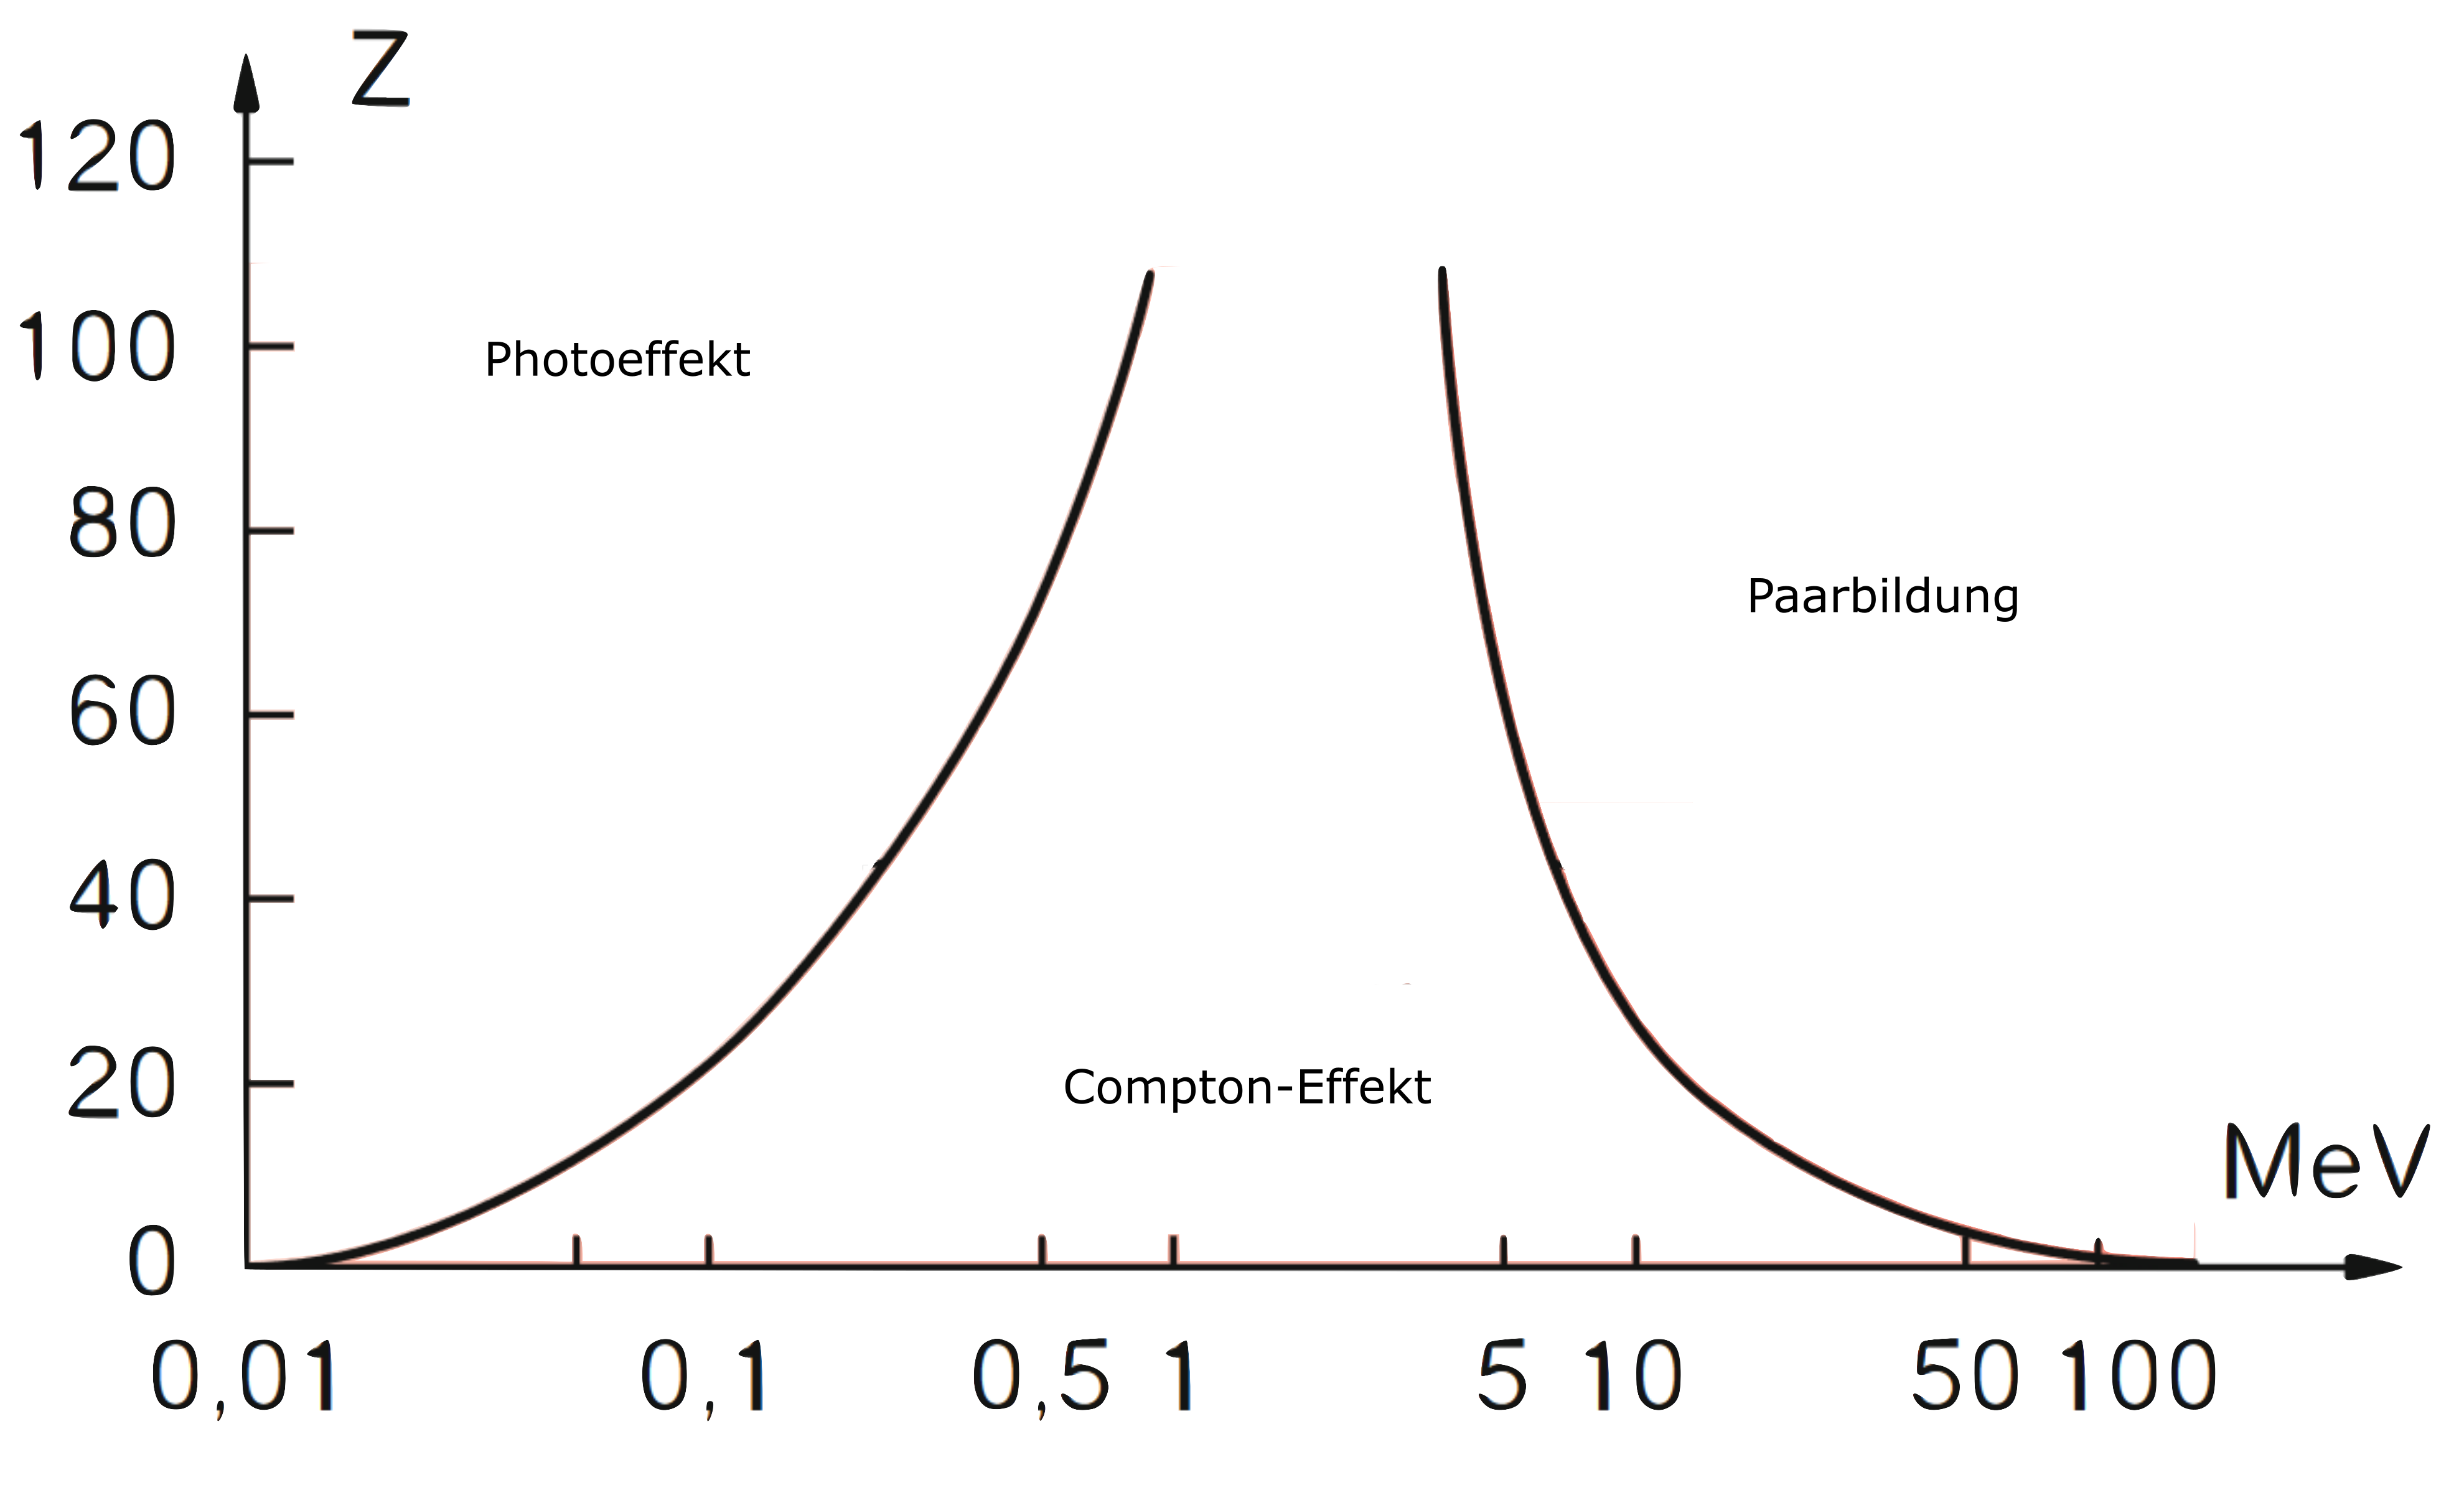
\includegraphics[scale=0.25]{PhotoQuerschnitte.png}
		\caption{Dominante Wechselwirkungen von Photonen in Abhängigkeit von der Kernladungszahl $Z$ des Absorbermaterials und der Photonenenergie. Die durchgezogenen Linien markieren die Grenzbereiche der dominierenden Effekte (modifiziert nach \cite{DemtroderKerne})}
		\label{fig:WirkungsquerschnittePhotonen}
	\end{figure}
	
		\subsubsection{Photoelektrischer Effekt}
		Der photoelektrische Effekt beschreibt die Absorption eines Photons durch ein gebundenes Elektron, wodurch das Atom angeregt oder ionisiert wird. Dieser Effekt dominiert im niederenergetischen Bereich (siehe Abbildung \ref{fig:WirkungsquerschnittePhotonen}). Mit der Bindungsenergie $\phi_{\text{A}}$ des Elektrons gilt für die Energie des auslösten Elektrons:
		\begin{equation*}
			E_{e^{-}}= E_{\gamma}-\phi_{\text{A}}
		\end{equation*} 
		
		\noindent Der Wirkungsquerschnitt ist sowohl kernladungszahl- als auch energieabhängig und tritt besonders stark bei Energien auf, die den Absorptionskanten der Atome entsprechen, insbesondere bei Atomen mit hoher Kernladungszahl  \cite{Leo}.
		
		
		\subsubsection{Compton-Streuung}
		Compton-Streuung ist die Streuung eines Photons an einem lose gebundenen Elektron. Ein Teil der Photonenenergie wird dabei auf das Elektron übertragen,das Photon wird nicht absorbiert. Man unterscheidet zwischen Rayleigh-, Thomson- und Compton-Streuung. Diese Phänomene werden durch die Klein-Nishina-Formel beschrieben, wobei die klassische Streuung den niederenergetischen Grenzfall der Compton-Streuung darstellt. Der Wirkungsquerschnitt der Compton-Streuung ist primär energieabhängig  \cite{Leo}:
		\begin{equation*}
			{\displaystyle \dv{\sigma}{\Omega}={\frac {1}{2}}{\frac {\alpha ^{2}}{m^{2}}}\left({\frac {E'}{E}}\right)^{2}\left({\frac {E'}{E}}+{\frac {E}{E'}}-\sin ^{2}\theta \right)}
		\end{equation*}
		wobei $\theta$ den Streuwinkel bezeichnet, $\alpha\approx 1/137$ die Feinstruktur-Konstante und $E^{\prime}$ die Energie des gestreuten Photons. Als ein Fall der elastischen Streuung existiert ein eindeutiger Zusammenhang zwischen der deponierten Energie und dem Streuwinkel.
		
		\subsubsection{Paarbildung}
		Photonen deren Energie einen Wert von $1,22\ \si{MeV}$ überschreiten, können sich im Feld eines Kerns zu Elektronen-Positronen-Paaren umwandeln. Eine Umwandlung ohne einen dritten Wechselwirkungspartner ist aufgrund der Impulserhaltung nicht möglich. Paarbildung wird damit nur für hochenergetische Strahlung relevant. Der Wirkungsquerschnitt skaliert mit \cite{DemtroderKerne}:
		\begin{equation*}
			\sigma \propto Z^{2}\ln(E_{\gamma})
		\end{equation*} 
		
		
	\newpage
	
	\subsection{Sekundärionisation}	
		Nach der Primärionisation durch das tatsächliche Detektionsereignis gibt es einige Effekte, die zu weiteren Ionisationen durch dasselbe Ereignis beitragen können. In diesem Zusammenhang spricht man von Sekundärionisationen. Ein Verständnis dieser Effekte ist fundamental für die korrekte Beurteilung der Arbeitsparameter von Detektoren (siehe Abschnitte [GAIN und ENERGIERES]).
		
		\subsubsection{Lokale Clusterbildung}
			Wir ein Elektron bspw. durch den Photoeffekt ausgelöst, hat dieses Elektron oft noch so viel Energie, dass weitere Stoßwechselwirkungen mit den Atomen zu Sekundärionisationen führen können. Es bildet sich ein Lokales Cluster aus Elektronen, die zu einem Detektionsereignis gehören, da der Auslösungsprozess so lange geht, bis die Energie des Elektrons für weitere Ionisationen nicht mehr ausreicht. Bei bekannter Ionisationsenergie des Mediums kann die Zahl der durch ein Detektionsereignis erzeugten Elektronen-Ionen-Paare kann wie folgt approximiert werden \cite{Sauli_Multiwire}:
			\begin{equation*}
				N_{\text{e}}=\frac{E_{\gamma}}{\phi_{\text{bind}}}
			\end{equation*}	
			Der Wert, der aus dieser Formel folgt ist offenbar ein Erwartungswert. Da die Wechselwirkungsprozesse statistischer Natur sind, müssen die daraus folgenden Unschärfen berücksichtigt werden.
		
		\subsubsection{Penning-Effekt}
			Man kann nun ein anderes Molekül in das Medium geben, dessen Ionisationsenergie unterhalb der Anregungsniveaus des ursprünglichen Mediums liegt. Auf diese Weise kann man die Energie, die in Anregungen \enquote{verloren} geht wiederum durch Stoßwechselwirkungen zwischen den Atomen im Elektronen-Ionen-Paare umwandeln. In dieser Gasmischung wird die Effektive Ionisationsenergie quasi heruntergesetzt, sodass mehr Ionisationen stattfinden. Man bezeichnet dieses Gas als Quencher und den illustrierten Effekt als Penning Effekt \cite{ottnad}.
			
		\subsubsection{Auger-Meitner-Effekt}
			Im Kontext des Photoeffektes ist es wahrscheinlich, dass das ausgelöste Elektron aus einer unteren Schale stammt. Neben der Rekombination unter Emission von Strahlung oder internen Übergängen unter Photonenemission ist auch ein strahlungsloser interner Übergang möglich. Dabei kann ein weniger stark gebundenes Elektron der äußeren Schalen auf die innere zurückfallen und ihre Energie an ein anderes Elektron im System abgeben, was zu einer weiteren Ionisation führen kann \cite{Sauli_Multiwire}. 
			
		\subsubsection{$\delta$-Elektronen und nicht-lokale Clusterbildung}
			Die statistische Natur der Wechselwirkungsprozesse erlauben es, dass ein ein hochenergetisches freies Elektron entstehen kann, das durch das Medium propagiert und in Übereinstimmung mit einer Modifizierten Bethe-Bloch-Formel \cite{Leo} Energie verliert. Hierbei können weitere Elektronen-Ionen-Paare erzeugt werden, die Position dieser Sekundärerzeugung muss allerdings nicht mit dem Ort der Primärionisation übereinstimmen, sondern kann deutlich entfernt stattfinden. Daher können mehrere Cluster entstehen, die zu einem Ereingnis gehören. Delta-Elektronen können daher nicht nur die Ortsauflösung des Detektors beeinflussen, sondern auch für größere Fluktuationen bei der Messung der deponierten Energie sorgen.
			
		\newpage	
		
	\section{Bewegungen von Ladungen}		
	Nachdem die Detektionsereignisse stattfanden und daher freie Elektronen-Ionen-Paare existieren, müssen diese Ausgelesen werden. Dafür müssen die Ladungen von der Rekombination aufgehalten und getrennt werden, weswegen die Bewegung von Ladungsträgern und damit verbundene Größen definiert und verstanden werden müssen.\\
	Die Bewegung eines Ladungsträgers setzt sich zusammen aus der Eigenbewegung des Teilchens, die durch zahlreiche Stöße in thermische Bewegung (Diffusion) übergeht und die Driftbewegung in elektromagnetischen Feldern.
	
		\subsection{Diffusion}	
		Ohne Elektrische Felder bewegt sich das Elektron entsprechend der Energie- und Impulserhaltung nach der Ionisationswechselwirkung. Durch die Stöße mit den Gasatomen wird die Bewegung verlangsamt und so umgelenkt, dass die Bewegung eines Elektronenensembles nunmehr ungerichtet ist, die Elektronenwolke diffundiert. Die Beschreibung dieser Prozesse im Rahmen der kinetischen Gastheorie zeigt, dass die räumliche Verteilung um den Primären Ionisationspunkt gauß'sch ist, wobei die räumliche Ausdehnung aus der Standardabweichung abgeschätzt werden kann \cite{Sauli_Multiwire}. Die Diffusionsbewegung begrenzt also die räumliche Auflösung des Detektors auf natürliche Weise.\\
		\\
		Die Bewegung des Teilchens lässt sich durch die mittlere freie Weglänge beschreiben, die als Maß für die Strecke fungiert, die ein Teilchen zwischen zwei Wechselwirkungen zurücklegt. Sie ergibt sich aus der Teilchendichte $n$ und dem Wirkungsquerschnitt $\sigma$ über:
		\begin{equation}
			\lambda=\frac{1}{n\sigma}
		\end{equation} 
		Insbesondere lässt sich die mittlere freie Weglänge als Maß für die Interaktionsrate für Ionisation und Rekombination verwenden \cite{Sauli_Multiwire}. Für Elektronen ist die thermische Geschwindigkeit und die Mittlere Freie Weglänge mehrere Größenordnungen größer als für Ionen, es ist daher deutlich angemessener die Elektronen für die Signalerzeugung am Detektor zu Verwenden.
		
		\subsection{Bewegung von Ladungsträgern in Feldern}\label{sec:Bewegung in Feldern}
		Auf bewegte Ladungen in elektromagnetischen Feldern wirkt die Lorentzkraft und beschleunigt das Elektron entlang oder senkrecht zur Bewegungsrichtung. In der folgenden Detektorkonfiguration (siehe Abschnitt [GEM Design]) wird kein magnetisches Feld verwendet. Daher wird im Folgenden der Spezialfall mit Lorentzkraft für $\vec{B}=0$ betrachtet. Die Bewegung setzt sich zusammen aus den Stößen mit den Gasatomen und dem Drift im elektrischen Feld, das Problem wird damit beschrieben durch einen Spezialfall der Langevin-Gleichung \cite{Schwabl}:
		\begin{equation*}
			m \dot{v}= q \vec{E}- f(t)
		\end{equation*}
		Wobei $m$ die Teilchenmasse, $q$ die Ladung und $\vec{E}$ das elektrische Feld beschreibt, während $v$ die Geschwindigkeit und $f(t)$ eine zeitabhängige Kraft ist, die aus den Stoßwechselwirkungen resultiert. Man kann nun aus den Eigenschaften an die zeitbahängige Kraft Bedingungen konstruieren, die auf folgenden Zusammenhang für die Dirftgeschwindigkeit führen:
		\begin{equation*}
			\vec{v}= \mu \vec{E}
		\end{equation*}
		Wobei man $\mu=q/m \tau$ als Beweglichkeit des Teilchens bezeichnet, die mit der mittleren Stoßzeit $\tau$ und so mit der mittleren freien Weglänge zusammenhängt \cite{ottnad}. In erster Näherung wird damit klar, dass die Geschwindigkeit und so die kinetische Energie ausschlißelich vom anliegenden Elektrischen Feld abhängt.
		
		\newpage
	\section{Gasdetektorklassen}
		Mit den Eigenschaften um die Erzeugung und den Transport von Elektronen-Ionen-Paaren in Gasen können nun grundsätzliche Gasdetektorklassen abgeleitet werden, die sich vom grundlegenden Aufbau nicht sonderlich unterscheiden, sondern sehr wesentlich im Betrieb \cite{Leo}.
		
		\subsection{Ladungsmultiplikationsmechanismen} \label{sec:Ladungsmultiplikation}
			Wenn die kinetische Energie eines Teilchens die Ionisationsenergie eines Atoms überschreitet, kann es passieren, dass das Atom ionisiert wird. Ausgehend davon, dass die kinetische Energie geladener Teilchen in Feldern vom anliegenden Feld abhängt (siehe Abschnitt \ref{sec:Bewegung in Feldern}), kann das Feld so stark eingestellt werden, dass Sekundärionisationen stattfinden, wobei weitere Ionisationen je nach Größe der Region des starken Feldes möglich sind, insbesondere können dann auch in derselben Region ausgelöste Elektronen bereits zur Verstärkung der Elektronenwolke beitragen, es entsteht eine Lawine \cite{Townsend}, \cite{Leo}.\\
			\\
			Die Zahl der Ladungsträger, die pro Längeneinheit entstehen sind eng mit der Zahl der Wechselwirkungen und damit mit der mittleren freien Weglänge verbunden. Man bezeichnet die Zahl der entstehenden Ladungsträger als ersten Townsend-Koeffizienten, für den gilt:
			\begin{equation*}
				\alpha=\frac{1}{\lambda}
			\end{equation*}
			Die Wachstum der Elektronenlawine ist offenbar ein exponentieller Prozess, wobei der Townsend-Koeffizient sowie die Länge der Lawinenentstehungsgebietes relevante Größen sind, um die Lawinenentstehung zu beschreiben. Als Multiplikationsparameter wird die Verstärkung (im Folgenden Gain) definiert, die die Zahl der entstehenden Ladungen beschreibt:
			\begin{equation}
				G=\frac{N}{N_{0}} = e^{\alpha d}
			\end{equation}
			Der erste Townsendkoeffizient ist abhängig vom verwendeten Medium und steigt mit der Feldstärke an. Um Gasentladungen zu verhindern, kann die Zahl der Elektronen in diesem Volumen nicht beliebig ansteigen. Ein empirisch bestimmtes Limit für einen stabilen Betrieb ist das Raether-Limit nach dem gilt $\alpha d<20$ \cite{Sauli_Multiwire}.
			
		\subsection{Ionisations- und Proportionalkammern}
			Auf Basis der Ladungsmultipikationsmechanismen als Funktion des anliegenden Feldes ist es nunmehr möglich die beiden für diese Arbeit relevanten Detektorklassen zu definieren, da die Kenntnis über diese Systeme die Funktionsweise von GEM-Detektoren erheblich erleichtern wird.\\
			\\
			 Ionisationskammern sind gasgefüllte Kammern an denen ein elektrisches Feld anliegt, welches so stark ist, dass (fast) alle Ladungsträger gesammelt werden können, ohne allerdings eine Verstärkung zu erzeugen. Ionisationskammern können für geladene Teilchen zur Spurrekonstruktion genutzt werden, indem die Ausleseelektronik entsprechend segmentiert wird und die auftreffenden Elektronen auf der Auslese lokalisiert werden. Ein dreidimensionales Bild kann dann aus der zweidimensionalen Projektion aus der Auslesestruktur und der Zeit zwischen den Detektionsereignissen gewonnen werden. [ZITAT????] Das Feld und damit die Zeitauflösung ist nach oben hin durch das Ladungsmultiplikationsregime begrenzt.\\
			 \\
			 Proportinalkammern sind Gasgefüllte Kammern, die von einem Elektrischen Feld durchzogen sind, die so stark sind, dass Ladungsmultiplikation stattfinden kann. In Abbildung [ABBBILDUNG] ist die Feldabhängigkeit für eine Gasmischung aus Argon und $\text{CO}_{2}$ zu sehen. Demnach beginnt das Multiplikationsregime bei [ZAHLENWERT], sodass eine untere Grenze für die Felder existiert. Das Problem mit einer Proportionalkammer ist, dass in dem bisherigen Setup der Ort der Ionisation für die Verstärkung relevant ist, durch eine Verknüpfung mit einer Ionisationskammer kann die Ionisationsregion von der Verstärkungsregion getrennt werden, wodurch das Problem gelöst ist. Hat das anliegende Feld eine Größenordnung, die die Zahl der entstehenden Ionen moderat hält, dann ist die Zahl der emittierten Elektronen proportional zur Zahl der einfallenden Elektronen.
			 
		\subsection{Parameter von Gasdetektoren}
			Zum Abschluss des Grundlagenkapitels für Gasdetektoren sollen nun einige finale Überlegungen zu generellen Eigenschaften und Parametern von Gasdetektoren angestellt werden. Im folgenden werden demnach die Ionisationseigenschaften des Aktiven Mediums, sowie die Energieauflösung von Gasdetektoren diskutiert,
			
			\subsubsection{Wahl des Gases}
				Unterschiedliche Moleküle haben unterschiedliche Ionisationsenergien und daher unterschiedliche, elementspezifische Townsend-Koeffizienten. Die Verstärkung ist demnach abhängig von der Wahl des Aktiven Mediums und ist ihrerseits Thema kontinuierlicher Untersuchung \cite{GAS_MIX}. Neben einer möglichst geringen Ionisationsenergie sind weitere praktische Überlegungen für die Wahl des Arbeitsmediums anzustellen. Zum einen sollte das Medium reaktionsträge sein, da Alterungserscheinungen auf diese Weise später auftreten [QUELLE], die Wahl fällt demnach idealerweise auf ein Edelgas. Ferner sollten die mittlere freie Weglänge sowie die Driftgeschwindigkeit im Medium so dimensioniert sein, dass die Elektronen die Ionisationsregion schnell verlassen und so zeitnah zur Signalerzeugung beitragen.\\
				\\
				Um eine möglichst große Elektronenausbeute zu garantieren, wird im folgenden Argon verwendet, das Argon vergleichsweise niedrige Ionisationsenergien hat (siehe Tabelle \ref{tab:Ionisationsenergien}), wobei CO$_{2}$ als Quench-Gas beigemischt wird. Das Mischungsverhältnis der Gase wird im Folgenden $90-10$ sein, dies erlaubt eine adäquate Ausnutzung der in [ABSCHNITT] erwähnten Effekte.
				
				\begin{table}[h]
					\centering
					\begin{tabular}{|c|c|c|c|c|c|c|c|c|}
						\hline
						Gas & He & Ne & Ar & Kr & Xe & \ce{CO_{2}} & \ce{CH_{4}} & $\ce{Ar-CO_{2}} (90-10)$\\
						\hline
						$W_{\text{ion}} / \si{eV}$ & 42,7 & 36,8 & 26,4 & 24,1 & 21,9 & 34,5 & 29,2 & 27,2\\
						\hline
					\end{tabular}
					\caption{mittlere Ionisierungsenergie für ausgewählte Gase nach \cite{Gas_Energien} }
					\label{tab:Ionisationsenergien}
				\end{table}
				
				
			\subsubsection{Energieauflösung eines Detektors}
				Die Strahlung, die bei Kernprozessen emittiert wird ist diskret. Idealerweise ist die Strahlung hierbei monochromatisch, wobei die natürliche Linienbreite zu beachten ist. Detektoren werden die Linien dabei im Allgemeinen nicht so genau nachweisen können, sie haben eine intrinsiche Energeiauflösung. Die Energieauflösung bei Gasdetektoren setzt sich im Wesentlichen aus zwei Anteilen zusammen:
				\begin{enumerate}
					\item Ionisationsfluktuationen: Die Primärionisationsvorgänge sind bekanntermaßen ein statisticher Prozess. Da die Ereignisse nicht gänzlich statistisch unabhängig sind [ZITAT], muss die Standardabweichung der Poission-Verteilung um den Fanofaktor korrigiert werden, es ergibt sich ein Anteil zur Auflösung der folgenden Form:
					\begin{equation*}
						R=\frac{\sqrt{F}}{N}
					\end{equation*}
					\item Verstärkungsfluktuationen: Auch die Sekundärionisationsprozesse sind statistische Prozesse, die sehr wesentlich fluktuieren können, sodass sie einen signifikaten Einfluss auf die Auflösung hat. Es ergibt sich ein Anteil der folgenden Form:
					\begin{equation*}
						R= 
					\end{equation*}
				\end{enumerate}
				Man kann nun beide Anteile komninieren, und so eine Abschätzung  für die Gesamtenergieauflösung zu erhalten. Experimentell bestimmt sich die Energieauflösung durch die Auswertung eines wohlbekannten Spektrums [EISENSPEKTRUM], bei dem man eine bekannte Linie messen kann, um anschließend eine Kurve daran anzupassen und aus der Halbwertsbreite folgende Abschätzung zu verwenden:
				\begin{equation*}
					R=\frac{\Delta E}{E}= \frac{\sigma_{K_{\text{alpha}}}}{\mu_{K_{\alpha}}}
				\end{equation*}
				Eine Beschreibung der hier verwendeten Formelzeichen zur experimentellen Bestimmung findet sich in Kapitel [FESPEKTRUM]
			
			

\chapter{Gas Electron Multiplier}
Ordinäre Proportionalkammern sind natürlichen Problemen und Limitationen unterworfen. Beispielsweise sind die erreichbaren Verstärkungen durch das Raether-Limit oder durch die Proportionalitätsgrenzen der Kammer beschränkt, da sich sonst Raumladungen bilden, die aus Ionen bestehen und durch die Kammer propagieren, während sie das Feld in einer Form verzerren, die eine Multiplikation unmöglich macht. Der Ansatz, mit dem sich das Problem lösen lässt, ist die Einführung einer speziellen Detektorgeometrie. Eine Realisation dieser Geometrie sind die Multi-wire-proporional Chambers (MWPC), deren Funktionsweise extensiv in \cite{Sauli_Multiwire} diskutiert wird. 		In dieser Arbeit wollen wir eine andere Detektorgeometrie untersuchen, die Gas Electron Multiplier (GEM), die in diesem Kapitel eingeführt werden sollen:			 
				
\section{Aufbau und Funktionsweise einer GEM-Verstärkungsstufe}
GEM-Verstärkungsstufen sind dünne Isolatorfolien bestehend aus Polymiden, an deren Ober- und Unterseite eine Kupferbeschichtung anliegt. Um eine Nutzbarkeit als Verstärkerstufe zu gewährleisten werden Löcher in diese Platte geätzt, es ergibt sich eine Hexagonale Struktur wie in Abbildung \ref{fig:Draufsicht}. Mit der Hexagonalen Struktur ist der Abstand zweier Benachbarter Löcher paarweise gleich, dieser Abstand wird im folgenden als Pitch bezeichnet. Die Eigenschaften der Foliengeometrie wurden in der Vergangenheit bereits extensiv studiert \cite{Sauli_Übersicht}, auf Basis dieser Untersuchungen haben sich spezielle Konfigurationen etabliert, entsprechend dieser Konvention werden für diese Folien GEM-Folien im Standardformat verwendet, die Parameter der Folie sind als Querschnitt der Folie in Abbildung \ref{fig:Querschnitt} zu sehen.

	\begin{figure}[h]
		\centering
		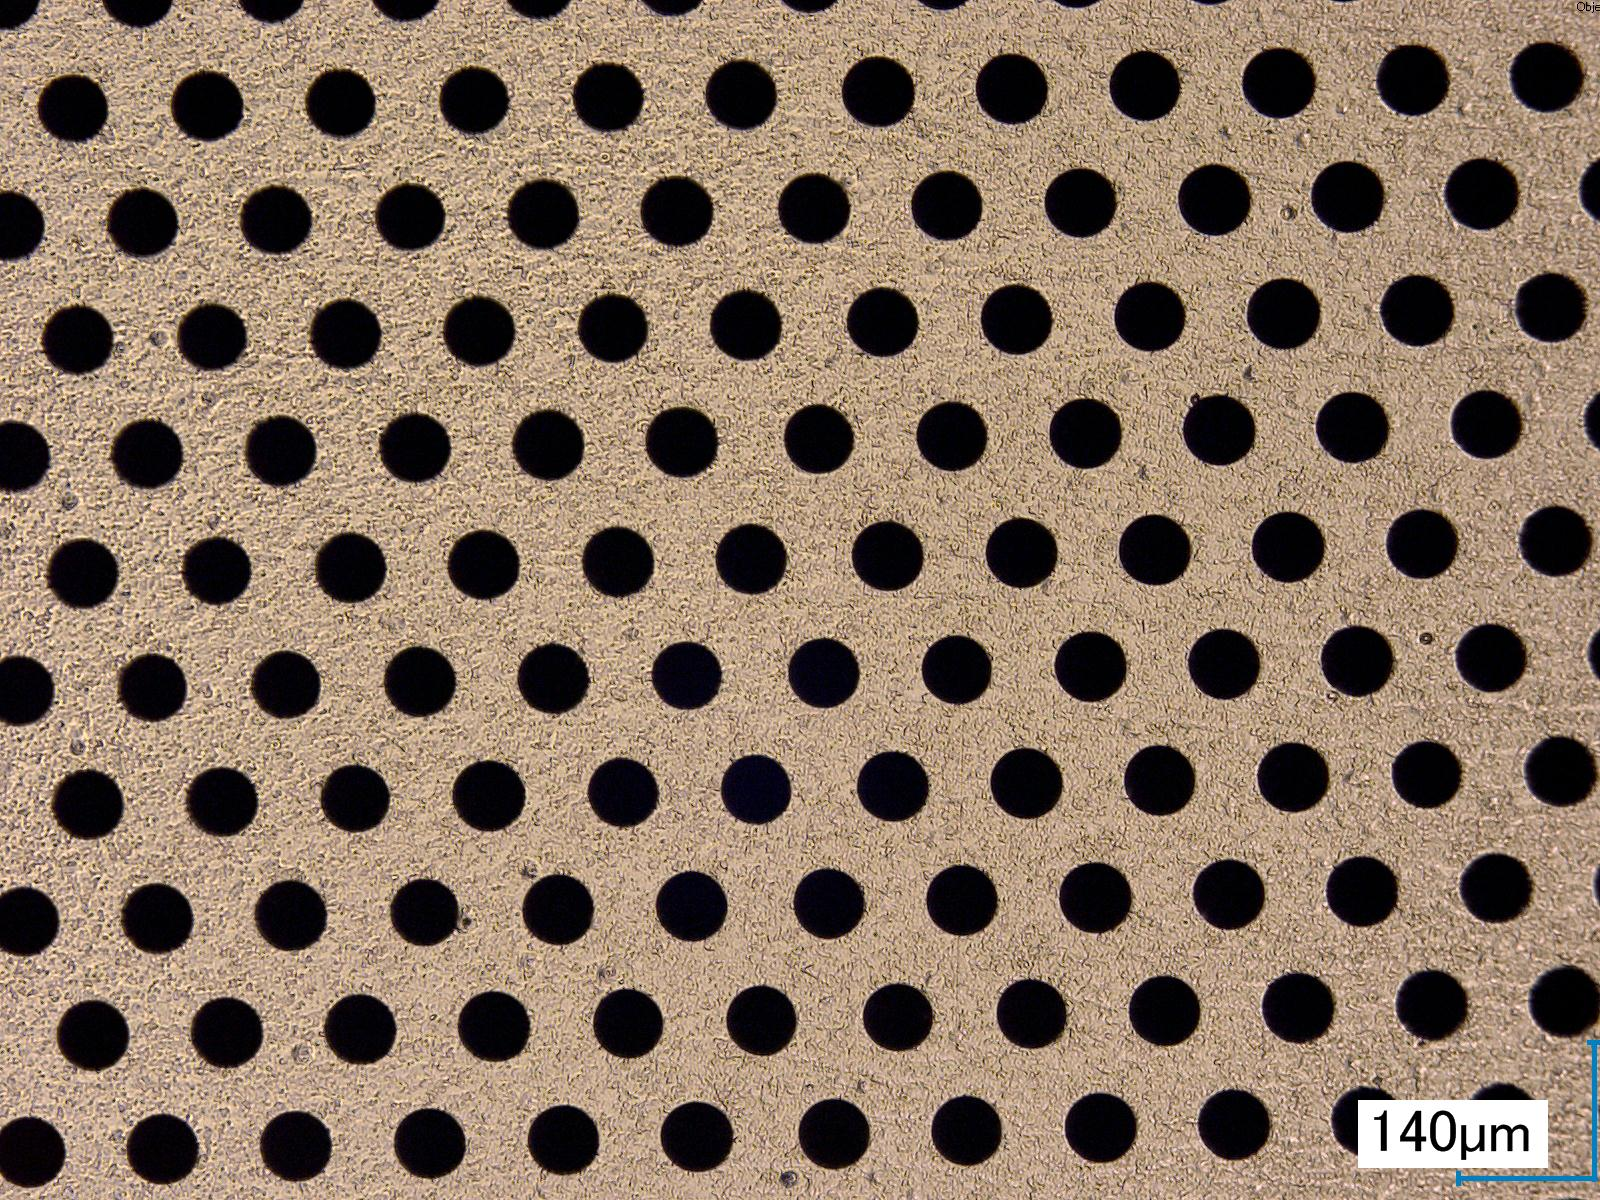
\includegraphics[scale=0.15]{Topside_UpperLeft.jpg}
		\caption{Draufsicht auf einen Folienausschnitt aufgenommen mit einem Mikroskop [MODELL?], ausgezeichnet ist der ein Maßstab von $140 \si{\mu m}$}
		\label{fig:Draufsicht}
	\end{figure}

	\begin{figure}[h]
		\centering
		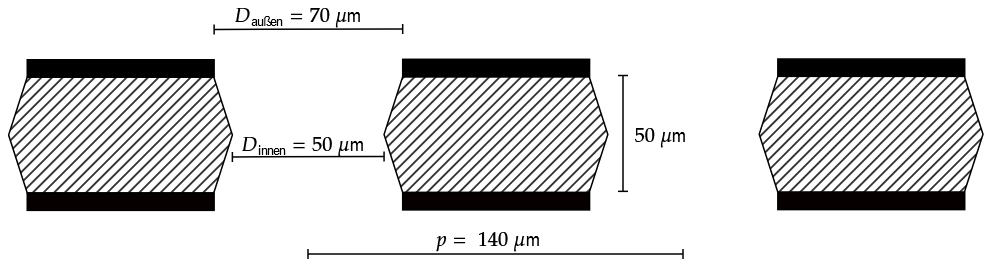
\includegraphics[scale=0.5]{Querschnitt GEM.png}
		\caption{Querschnitt der Folie}
		\label{fig:Querschnitt}
	\end{figure}
		
		
		
\noindent Legt man an die Kupferdecken eine Spannung an, wird in den Löchern ein starkes Feld induziert, legt man eine Spannung von $100 V$ an die GEM-Folie an, wird in den Löchern ein Feld der Größenordnung von $20.000\ \si{V/cm}$ induziert. Diese Felder sind hinreichend stark, um die in Absatz \ref{sec:Ladungsmultiplikation} diskutierten Ladungsmultipliationsmechanismen auszulösen. Es ist daher einzusehen, dass die Signalverstärkung in einer GEM-Stufe mit vergleichsweise geringem Aufwand potentiell sehr groß werden kann; es ist daher zum Zwecke eines stabilen Betriebes als Proportionalverstärker darauf zu achten, die Gain nach oben zu limitieren. Es ist in diesem Zusammenhang dennoch möglich, dass durch die statistische Verteilung der Energien der Primärelektronen Gasentladungen in den Folien zu Tage treten können. Diese können durch den Detektor propagieren und die Folie oder die Periphäre Ausleseelektronik beschädigen. Es ist daher angemessen die Ausleseelektronik hinreichend weit von der Verstärkung zu entfernen und ein deutlich schwächeres Feld zu verwenden, um die Elektronenwolke zur Ausleseelektronik zu befördern, wo dann ein Signal induziert wird. Schematisch ergibt sich eine Struktur wie in Abbildung
			



\section{Multi-GEM-Strukturen}
Ähnlich zu den einfachen Proportionalkammern haben Single-GEM-Detektoren wesentliche Gain Limitationen. Möchte man höhere Verstärkungen bei stabilerem Betrieb erreichen, kann man mehrere Verstärkerstufen hintereinander betreiben. Je nach Abstand der Folien, können Diffusionseffekte dafür sorgen, dass Elektronen, die aus einem GEM-Folienloch ausgegeben werden in mehreren GEM-Löchern der Folgefolie verstäkrt werden. Auf diese Weise wird das Raether-Limit, welches für eines der GEM-Löcher gilt umgangen.\\
Es ist ferner so, dass die Spannungen die an einer Folie angelegt werden reduziert werden können, um dennoch dieselbe Verstärkung zu erreichen. Die Nutzung mehrerer Stufen erlaubt also einen Stabileren Betrieb, da die Discharge-Wahrscheinlichkeit erheblich sinkt. [GAIN-PLOTS]. Die Übergabe der Elektronen von einer Folie zur anderen erfolgt dabei über die Transferfelder. Während es potentiell möglich ist eine große Zahl von Folien zu verwenden, bietet es sich an eine Konstallation genauer zu unteruschen, die Triple-GEM-Detektoren. Der schematische Aufbau eines solchen Detektors ergibt sich aus Abbildung [SCHEMATIC].\\
IONEN-BACKFLOW

\section{Effektive Gain und Transfereffizienzen}
In einem Idealen System würden alle Elektronen, die bei der Verstärkung erzeugt werden auch in die nächste Verstärkerstufe und so zur Ausleseelektronik gelangen. In der Praxis ergeben sich im Wesentlichen drei Wege, über die Elektronen für die anderen Stufen verloren gehen können:
\begin{enumerate}
	\item Wechselwirkung mit der oberen Kupferplatte: Die Elektronen werden von dem GEM-Feld im Allgemeinen in das Loch gesaugt, es gibt jedoch einen Teil der Elektronen, die nicht eingesaugt werden, sondern von der Kupferplatte abgefangen werden. Diese Elektronen stehen offenbar nicht mehr für die Verstärkung zur Verfügung
	\item Verluste durch Polymid-Interaktion: Elektronen, die in die Verstärkerstufe aufgenommen wurden, können von der Berandung der Löcher aufgenommen werden und stehen so nicht mehr zur Verfügung
	\item Wechselwirkungen mit der unteren Kupferplatte: Die Elektronen, die aus der Verstärkerstufe extrahiert werden, können bei der Extrahktion durch das GEM-Feld auf die untere Platte beschleunigt werden. Diese können dann offenbar nicht mehr weiterverwendet werden. 
\end{enumerate}
Physikalisch steht dahinter die Intuition, ob die Felder in einer Art zusammenwirken, die die Übergabe der Elektronen der Drift- und Transferfelder an GEM-Stufen begünstigen oder erschweren. Zu diesem Zweck definieren wir die Transfereffizienzen:
\begin{equation*}
	\epsilon_{\text{coll}}=\frac{N_{\text{gesammelt}}}{N_{\text{ein}}} \quad \epsilon_{\text{extr}}=\frac{N_{\text{extr}}}{N_{\text{extr}}+N_{\text{verl}}}
\end{equation*}
Hierbei bezeichnet die Kollekttionseffizienz $\epsilon_{\text{coll}}$ die Zahl der aus einer Stufe eingesammelten Ladungen normiert auf die Zahl der gesamt-einfallenden Ladungen und die Extraktionseffizienz $\epsilon_{\text{extr}}$ das Verhältnis der extrahierten Ladung normiert auf die Gesamtladung, die sich aus der extrahierten und der verlorenen Ladung zusammensetzt. Die Transfereffizienten verändern dabei offenbar die Verstärkung. Unter der Annahme, dass eine GEM-Stufe eine Absolute Verstärkung $G_{\textbf{abs}}$ hat, ergibt sich unter Verwendung der Transfereffizienzen folgender Zusammenhang:
\begin{equation}
	G_{\text{eff}}= \epsilon_{\textbf{coll}} \epsilon_{\text{extr}} G_{\text{abs}}
\end{equation}
Die effektive Verstärkung ist hierbei offenbar die Messbare Quantität (siehe Abschnitt Optimierungsroutine). Ein Vergleich der Größen findet sich in [ABBILDUNG]